\SetVertexStyle[Shape=circle, InnerSep=2, MinSize=14, FillColor=orange!40, LineColor=black, TextFont=\normalsize]
\SetEdgeStyle[Color=gray, Arrow=-stealth]

\begin{tikzpicture}
	\Vertex[x=-0.85, y=1.59, label=$A$]{0}
	\Vertex[x=-1.62, y=2.65, label=$B$]{1}
	\Vertex[x=3.00, y=-1.13, label=$C$]{2}
	\Vertex[x=2.1, y=-0.75, label=$D$]{3}
	\Vertex[x=0.40, y=1.67, label=$E$]{4}
	\Vertex[x=0.07, y=0.41, label=$F$]{5}
	\Vertex[x=-1.04, y=0.51, label=$G$]{6}
	\Vertex[x=1.34, y=0.97, label=$H$]{7}
	\Vertex[x=-0.9, y=-0.97, label=$I$]{8}
	\Vertex[x=-1, y=-2.12, label=$J$]{9}
	\Vertex[x=0.94, y=-0.52, label=$K$]{10}
	\Vertex[x=0.84, y=-1.66, label=$L$]{11}
	\Vertex[x=-2.11, y=-1.02, label=$M$]{12}
	\Edge[Direct, color=SentimentMissing](0)(0)
	\Edge[Direct, color=SentimentPositive](0)(1)
	\Edge[Direct, color=SentimentPositive, bend=-33](2)(3)
	\Edge[Direct, color=SentimentPositive, bend=33](2)(3)
	\Edge[Direct, color=SentimentMissing](4)(5)
	\Edge[Direct, color=SentimentMissing](0)(5)
	\Edge[Direct, color=SentimentNegative](6)(5)
	\Edge[Direct, color=SentimentPositive](7)(5)
	\Edge[Direct, color=SentimentNeutral](8)(9)
	\Edge[Direct, color=SentimentNeutral](10)(11)
	\Edge[Direct, color=SentimentNegative](10)(5)
	\Edge[Direct, color=SentimentNeutral, bend=-33](10)(5)
	\Edge[Direct, color=SentimentMissing, bend=33](10)(5)
	\Edge[Direct, color=SentimentMissing](10)(3)
	\Edge[Direct, color=SentimentMissing](8)(5)
	\Edge[Direct, color=SentimentNegative](8)(12)
\end{tikzpicture}
